\chapter{Software Requirement Specifications}
\label{ch:srs}
This chapter specifies the requirements of the FaceCon system. FaceCon is a research and development pipeline with a demonstration front end rather than a conventional multi-user application, so its users are the researcher-developer who builds and runs the pipeline, the evaluator who inspects the results, and a demonstration user who views predicted faces. The chapter sets out the system features, the functional and non-functional requirements, the quality attributes, the assumptions, the use cases, the hardware and software requirements, the user interface, the data design, and a risk analysis. Each requirement is written so that it is specific, testable, and traceable to the methodology and design that follow.

\section{List of Features}
The system provides the following features.
\begin{itemize}
\item F1. Ingest genotype data, build a subject by SNP dosage matrix, and apply documented QC.
\item F2. Reduce the genotypes that pass QC to a documented, GWAS-informed SNP panel.
\item F3. Ingest 3D scans and demographics, and register scans to FLAME to export shape parameters.
\item F4. Pair subjects that have both a valid genotype and a valid FLAME target.
\item F5. Train demographics only, SNP only, and combined predictive models through a baselines first progression.
\item F6. Decode predicted FLAME parameters into a 3D mesh.
\item F7. Evaluate predictions with FLAME parameter, mesh, landmark, region, and retrieval metrics.
\item F8. Compare against mean face and demographic baselines and run SNP panel ablations.
\item F9. Export meshes, metrics, and plots, and provide a demonstration interface for predicted and baseline faces.
\item F10. Integrate an established forensic DNA phenotyping method (HIrisPlex-S) that uses the same genotype to provide eye colour, hair colour, and skin colour alongside the reconstructed face.
\item F11. Render the predicted skin colour and eye colour on the reconstructed face and report hair colour, rendering it only where suitable hair geometry exists.
\end{itemize}

\section{Functional Requirements}
The functional requirements describe the external behaviour of the system and are stated as testable ``shall'' requirements.
\begin{itemize}
\item FR-01. The system shall ingest genotype data and construct a subject-by-SNP allele-dosage matrix.
\item FR-02. The system shall perform genotype QC, including filtering by missingness, minor-allele frequency, Hardy--Weinberg equilibrium, and relatedness, and shall produce a documented SNP panel.
\item FR-03. The system shall ingest 3D facial scans and their associated demographic attributes.
\item FR-04. The system shall register facial scans to the FLAME model and export FLAME shape and identity parameters as prediction targets.
\item FR-05. The system shall match subjects that have both a valid genotype and a valid FLAME target, and shall generate subject-level training, validation, and test splits.
\item FR-06. The system shall train and run predictive models, including demographics-only, SNP-only, and combined genotype and demographics models.
\item FR-07. The system shall decode predicted FLAME parameters into a 3D facial mesh.
\item FR-08. The system shall evaluate predictions using FLAME-parameter, per-vertex mesh, landmark, region-level, and retrieval metrics.
\item FR-09. The system shall compare model predictions against mean-face and demographic baselines, and shall support SNP-panel ablation experiments such as GWAS-informed versus matched-random panels.
\item FR-10. The system shall export predicted meshes, metric tables, and plots, and shall provide a local demonstration interface for viewing predictions.
\item FR-11. The system shall extract the HIrisPlex-S marker SNPs from the same genotype used for shape prediction and obtain eye colour, hair colour, and skin colour from the established HIrisPlex-S predictor, without training a new appearance model.
\item FR-12. The system shall pass the HIrisPlex-S colour outputs to the visualization layer, rendering skin colour and eye colour on the reconstructed face and reporting hair colour (rendered only where suitable hair geometry exists).
\end{itemize}

\section{Quality Attributes}
The system is designed around six quality attributes. Reproducibility means that every result can be regenerated from recorded code, configuration, and random seeds. Transparency means that all data-processing and SNP-selection decisions are documented. Correctness means that numerical pipelines are validated against known inputs. Efficiency means that the core baselines run on commonly available development hardware. Usability means that the demonstrator can be operated by a non-expert evaluator. Maintainability means that the code is modular, so that stages can be replaced independently.

\section{Non-Functional Requirements}
The non-functional requirements constrain how the system behaves and are likewise written as testable ``shall'' statements.
\begin{itemize}
\item NFR-01. The system shall use strictly subject-level training, validation, and test splits, with no subject appearing in more than one split.
\item NFR-02. The system shall fit any dataset-derived SNP-selection and normalization statistics using training data only.
\item NFR-03. The system shall be configuration-driven, so that every experiment can be reproduced from a stored configuration and random seed.
\item NFR-04. The system shall allow model complexity to be matched to the final paired sample size.
\item NFR-05. The system's preprocessing, QC, and baseline models shall be executable on standard development hardware, while more computationally demanding neural training shall be able to run on higher-capacity GPU resources such as those provided by shared or institutional computing facilities.
\item NFR-06. The system shall support honest reporting, including repeated evaluation or confidence estimates where feasible, and shall not present results that overstate predictive performance.
\item NFR-07. The system shall handle controlled genetic and biometric data strictly under the approved data-use agreement, and shall not expose raw individual-level data or permit re-identification.
\end{itemize}

\section{Assumptions}
The specification makes several assumptions. It assumes that controlled-access approval for the dbGaP genotypes and FaceBase scans is granted within the project timeline, and that a workable number of subjects have both genotype and 3D-scan data. It assumes that FaceBase scans can be registered to FLAME with acceptable fitting error. Finally, it assumes that published facial-GWAS results are at least approximately applicable to the ancestry composition of the cohort.

\section{Use Cases}
\label{sec:usecases}
This section presents the use cases of the system in the standard tabular format, each identified by a use-case number. The first three use cases concern the research pipeline: UC-01 builds the SNP panel (Table~\ref{tab:uc1}), UC-02 fits a scan to FLAME (Table~\ref{tab:uc2}), and UC-03 predicts and evaluates a face from a genotype (Table~\ref{tab:uc3}). The remaining three concern the demonstrator and correspond directly to the interface screens of Section~\ref{sec:gui}: UC-04 selects a held-out test subject (Table~\ref{tab:uc4}), UC-05 views the prediction (Table~\ref{tab:uc5}), and UC-06 views the evaluation and results (Table~\ref{tab:uc6}).

\begin{table}[!ht]
\centering
\caption{UC-01: perform genotype QC and build the SNP panel.}
\label{tab:uc1}
\begin{tabular}{|lllll|}
\hline
\multicolumn{2}{|l|}{\textbf{Use Case ID}} & \multicolumn{3}{l|}{UC-01} \\ \hline
\multicolumn{2}{|l|}{\textbf{Name}} & \multicolumn{3}{l|}{Perform Genotype QC and Build SNP Panel} \\ \hline
\multicolumn{2}{|l|}{\textbf{Actors}} & \multicolumn{3}{l|}{Researcher-Developer} \\ \hline
\multicolumn{2}{|l|}{\textbf{Summary}} & \multicolumn{3}{l|}{\begin{tabular}[c]{@{}l@{}}The developer ingests genotypes, applies documented QC filters, and\\ reduces the data to a GWAS-informed, documented SNP panel.\end{tabular}} \\ \hline
\multicolumn{2}{|l|}{\textbf{Pre-Conditions}} & \multicolumn{3}{l|}{\begin{tabular}[c]{@{}l@{}}Controlled-access genotype files are available locally within the\\ approved data-use agreement.\end{tabular}} \\ \hline
\multicolumn{2}{|l|}{\textbf{Post-Conditions}} & \multicolumn{3}{l|}{A QC report and a documented SNP-panel file are produced.} \\ \hline
\multicolumn{2}{|l|}{\textbf{Special Requirements}} & \multicolumn{3}{l|}{Processing stays within the data-use agreement.} \\ \hline
\multicolumn{5}{|c|}{\textbf{Basic Flow}} \\ \hline
\multicolumn{3}{|c|}{\textbf{Actor Action}} & \multicolumn{2}{c|}{\textbf{System Response}} \\ \hline
\multicolumn{1}{|l|}{1} & \multicolumn{2}{l|}{\begin{tabular}[c]{@{}l@{}}The developer supplies genotype\\ files and QC thresholds.\end{tabular}} & \multicolumn{1}{l|}{2} & \begin{tabular}[c]{@{}l@{}}The system validates inputs and\\ loads genotypes.\end{tabular} \\ \hline
\multicolumn{1}{|l|}{3} & \multicolumn{2}{l|}{The developer starts QC.} & \multicolumn{1}{l|}{4} & \begin{tabular}[c]{@{}l@{}}The system applies missingness, MAF,\\ HWE, and relatedness filters, logging\\ each step.\end{tabular} \\ \hline
\multicolumn{1}{|l|}{5} & \multicolumn{2}{l|}{\begin{tabular}[c]{@{}l@{}}The developer requests panel\\ construction.\end{tabular}} & \multicolumn{1}{l|}{6} & \begin{tabular}[c]{@{}l@{}}The system intersects QC-passed SNPs\\ with the GWAS-informed list and\\ exports the panel.\end{tabular} \\ \hline
\multicolumn{5}{|c|}{\textbf{Alternative Flow}} \\ \hline
\multicolumn{1}{|l|}{3-A} & \multicolumn{2}{l|}{Input is malformed.} & \multicolumn{1}{l|}{4-A} & \begin{tabular}[c]{@{}l@{}}The system reports the error and halts\\ without producing a panel.\end{tabular} \\ \hline
\end{tabular}
\end{table}

\begin{table}[!ht]
\centering
\caption{UC-02: register a scan to FLAME.}
\label{tab:uc2}
\begin{tabular}{|lllll|}
\hline
\multicolumn{2}{|l|}{\textbf{Use Case ID}} & \multicolumn{3}{l|}{UC-02} \\ \hline
\multicolumn{2}{|l|}{\textbf{Name}} & \multicolumn{3}{l|}{Register a Scan to FLAME} \\ \hline
\multicolumn{2}{|l|}{\textbf{Actors}} & \multicolumn{3}{l|}{Researcher-Developer} \\ \hline
\multicolumn{2}{|l|}{\textbf{Summary}} & \multicolumn{3}{l|}{\begin{tabular}[c]{@{}l@{}}The developer fits a FaceBase scan to FLAME to obtain a common\\ mesh and shape parameters.\end{tabular}} \\ \hline
\multicolumn{2}{|l|}{\textbf{Pre-Conditions}} & \multicolumn{3}{l|}{A valid scan and the FLAME model are available.} \\ \hline
\multicolumn{2}{|l|}{\textbf{Post-Conditions}} & \multicolumn{3}{l|}{FLAME shape parameters and a registered mesh are saved.} \\ \hline
\multicolumn{2}{|l|}{\textbf{Special Requirements}} & \multicolumn{3}{l|}{Fitting error must be below the configured threshold.} \\ \hline
\multicolumn{5}{|c|}{\textbf{Basic Flow}} \\ \hline
\multicolumn{3}{|c|}{\textbf{Actor Action}} & \multicolumn{2}{c|}{\textbf{System Response}} \\ \hline
\multicolumn{1}{|l|}{1} & \multicolumn{2}{l|}{The developer selects a scan.} & \multicolumn{1}{l|}{2} & \begin{tabular}[c]{@{}l@{}}The system loads the scan and\\ initializes FLAME fitting.\end{tabular} \\ \hline
\multicolumn{1}{|l|}{3} & \multicolumn{2}{l|}{\begin{tabular}[c]{@{}l@{}}The developer starts\\ registration.\end{tabular}} & \multicolumn{1}{l|}{4} & \begin{tabular}[c]{@{}l@{}}The system optimizes FLAME parameters\\ and reports the fitting error.\end{tabular} \\ \hline
\multicolumn{1}{|l|}{5} & \multicolumn{2}{l|}{The developer accepts the fit.} & \multicolumn{1}{l|}{6} & \begin{tabular}[c]{@{}l@{}}The system stores shape parameters and\\ the registered mesh.\end{tabular} \\ \hline
\multicolumn{5}{|c|}{\textbf{Alternative Flow}} \\ \hline
\multicolumn{1}{|l|}{4-A} & \multicolumn{2}{l|}{\begin{tabular}[c]{@{}l@{}}Fitting error exceeds the\\ threshold.\end{tabular}} & \multicolumn{1}{l|}{5-A} & \begin{tabular}[c]{@{}l@{}}The system flags the subject and excludes\\ it from training if unresolved.\end{tabular} \\ \hline
\end{tabular}
\end{table}

\begin{table}[!ht]
\centering
\caption{UC-03: predict and evaluate a face from genotype.}
\label{tab:uc3}
\begin{tabular}{|lllll|}
\hline
\multicolumn{2}{|l|}{\textbf{Use Case ID}} & \multicolumn{3}{l|}{UC-03} \\ \hline
\multicolumn{2}{|l|}{\textbf{Name}} & \multicolumn{3}{l|}{Predict and Evaluate a Face from Genotype} \\ \hline
\multicolumn{2}{|l|}{\textbf{Actors}} & \multicolumn{3}{l|}{Researcher-Developer, Evaluator} \\ \hline
\multicolumn{2}{|l|}{\textbf{Summary}} & \multicolumn{3}{l|}{\begin{tabular}[c]{@{}l@{}}The system predicts FLAME shape from a genotype, decodes a mesh,\\ and evaluates it against baselines.\end{tabular}} \\ \hline
\multicolumn{2}{|l|}{\textbf{Pre-Conditions}} & \multicolumn{3}{l|}{\begin{tabular}[c]{@{}l@{}}A trained model and a held-out test subject on the SNP panel\\ are available.\end{tabular}} \\ \hline
\multicolumn{2}{|l|}{\textbf{Post-Conditions}} & \multicolumn{3}{l|}{A predicted mesh and its baseline-relative metrics are produced.} \\ \hline
\multicolumn{2}{|l|}{\textbf{Special Requirements}} & \multicolumn{3}{l|}{No raw individual-level genotype is exposed in outputs.} \\ \hline
\multicolumn{5}{|c|}{\textbf{Basic Flow}} \\ \hline
\multicolumn{3}{|c|}{\textbf{Actor Action}} & \multicolumn{2}{c|}{\textbf{System Response}} \\ \hline
\multicolumn{1}{|l|}{1} & \multicolumn{2}{l|}{\begin{tabular}[c]{@{}l@{}}The user selects a held-out\\ test subject.\end{tabular}} & \multicolumn{1}{l|}{2} & \begin{tabular}[c]{@{}l@{}}The system predicts FLAME parameters\\ and decodes a mesh.\end{tabular} \\ \hline
\multicolumn{1}{|l|}{3} & \multicolumn{2}{l|}{\begin{tabular}[c]{@{}l@{}}The evaluator requests\\ evaluation.\end{tabular}} & \multicolumn{1}{l|}{4} & \begin{tabular}[c]{@{}l@{}}The system computes metrics and compares\\ against mean-face and demographic baselines.\end{tabular} \\ \hline
\multicolumn{5}{|c|}{\textbf{Alternative Flow}} \\ \hline
\multicolumn{1}{|l|}{2-A} & \multicolumn{2}{l|}{\begin{tabular}[c]{@{}l@{}}Genotype is missing\\ panel SNPs.\end{tabular}} & \multicolumn{1}{l|}{3-A} & \begin{tabular}[c]{@{}l@{}}The system imputes or masks missing SNPs\\ per the documented policy, or flags them.\end{tabular} \\ \hline
\end{tabular}
\end{table}

\begin{table}[!ht]
\centering
\caption{UC-04: select a held-out test subject.}
\label{tab:uc4}
\begin{tabular}{|lllll|}
\hline
\multicolumn{2}{|l|}{\textbf{Use Case ID}} & \multicolumn{3}{l|}{UC-04} \\ \hline
\multicolumn{2}{|l|}{\textbf{Name}} & \multicolumn{3}{l|}{Select a Held-Out Test Subject} \\ \hline
\multicolumn{2}{|l|}{\textbf{Actors}} & \multicolumn{3}{l|}{Demonstration User, Evaluator} \\ \hline
\multicolumn{2}{|l|}{\textbf{Summary}} & \multicolumn{3}{l|}{\begin{tabular}[c]{@{}l@{}}The user selects a preprocessed held-out test subject and initiates\\ a prediction from the demonstrator.\end{tabular}} \\ \hline
\multicolumn{2}{|l|}{\textbf{Pre-Conditions}} & \multicolumn{3}{l|}{\begin{tabular}[c]{@{}l@{}}A trained model and a set of preprocessed held-out test subjects\\ are available.\end{tabular}} \\ \hline
\multicolumn{2}{|l|}{\textbf{Post-Conditions}} & \multicolumn{3}{l|}{The subject is loaded and a prediction is requested.} \\ \hline
\multicolumn{2}{|l|}{\textbf{Special Requirements}} & \multicolumn{3}{l|}{No raw genotype information is displayed.} \\ \hline
\multicolumn{5}{|c|}{\textbf{Basic Flow}} \\ \hline
\multicolumn{3}{|c|}{\textbf{Actor Action}} & \multicolumn{2}{c|}{\textbf{System Response}} \\ \hline
\multicolumn{1}{|l|}{1} & \multicolumn{2}{l|}{\begin{tabular}[c]{@{}l@{}}The user selects a held-out\\ subject from the list.\end{tabular}} & \multicolumn{1}{l|}{2} & \begin{tabular}[c]{@{}l@{}}The system loads the subject's preprocessed\\ features, demographics, and ground truth.\end{tabular} \\ \hline
\multicolumn{1}{|l|}{3} & \multicolumn{2}{l|}{\begin{tabular}[c]{@{}l@{}}The user clicks\\ ``Generate Prediction''.\end{tabular}} & \multicolumn{1}{l|}{4} & \begin{tabular}[c]{@{}l@{}}The system initiates prediction and opens\\ the prediction-comparison view.\end{tabular} \\ \hline
\multicolumn{5}{|c|}{\textbf{Alternative Flow}} \\ \hline
\multicolumn{1}{|l|}{1-A} & \multicolumn{2}{l|}{No subject is selected.} & \multicolumn{1}{l|}{2-A} & \begin{tabular}[c]{@{}l@{}}The system keeps the button disabled and\\ prompts the user to select a subject.\end{tabular} \\ \hline
\end{tabular}
\end{table}

\begin{table}[!ht]
\centering
\caption{UC-05: view the prediction.}
\label{tab:uc5}
\begin{tabular}{|lllll|}
\hline
\multicolumn{2}{|l|}{\textbf{Use Case ID}} & \multicolumn{3}{l|}{UC-05} \\ \hline
\multicolumn{2}{|l|}{\textbf{Name}} & \multicolumn{3}{l|}{View the Prediction} \\ \hline
\multicolumn{2}{|l|}{\textbf{Actors}} & \multicolumn{3}{l|}{Demonstration User, Evaluator} \\ \hline
\multicolumn{2}{|l|}{\textbf{Summary}} & \multicolumn{3}{l|}{\begin{tabular}[c]{@{}l@{}}The user views the predicted FLAME face in an interactive viewer,\\ inspects the quantitative metrics, and compares the predicted mesh\\ with the ground truth.\end{tabular}} \\ \hline
\multicolumn{2}{|l|}{\textbf{Pre-Conditions}} & \multicolumn{3}{l|}{A prediction has been generated for the selected subject.} \\ \hline
\multicolumn{2}{|l|}{\textbf{Post-Conditions}} & \multicolumn{3}{l|}{\begin{tabular}[c]{@{}l@{}}The predicted mesh, its metrics, and the comparison with the\\ ground truth are displayed, and the evaluation and results view\\ can be opened.\end{tabular}} \\ \hline
\multicolumn{2}{|l|}{\textbf{Special Requirements}} & \multicolumn{3}{l|}{Faces are shown as FLAME geometry, not photographs.} \\ \hline
\multicolumn{5}{|c|}{\textbf{Basic Flow}} \\ \hline
\multicolumn{3}{|c|}{\textbf{Actor Action}} & \multicolumn{2}{c|}{\textbf{System Response}} \\ \hline
\multicolumn{1}{|l|}{1} & \multicolumn{2}{l|}{\begin{tabular}[c]{@{}l@{}}The user opens the\\ prediction view.\end{tabular}} & \multicolumn{1}{l|}{2} & \begin{tabular}[c]{@{}l@{}}The system renders the predicted mesh and\\ shows metrics and the predicted versus\\ ground truth comparison.\end{tabular} \\ \hline
\multicolumn{1}{|l|}{3} & \multicolumn{2}{l|}{\begin{tabular}[c]{@{}l@{}}The user rotates or zooms\\ the 3D viewer.\end{tabular}} & \multicolumn{1}{l|}{4} & \begin{tabular}[c]{@{}l@{}}The system updates the viewer in\\ real time.\end{tabular} \\ \hline
\multicolumn{5}{|c|}{\textbf{Alternative Flow}} \\ \hline
\multicolumn{1}{|l|}{3-A} & \multicolumn{2}{l|}{\begin{tabular}[c]{@{}l@{}}The user clicks ``View\\ detailed evaluation''.\end{tabular}} & \multicolumn{1}{l|}{4-A} & \begin{tabular}[c]{@{}l@{}}The system opens the evaluation and\\ results view (UC-06).\end{tabular} \\ \hline
\end{tabular}
\end{table}

\begin{table}[!ht]
\centering
\caption{UC-06: view the evaluation and results.}
\label{tab:uc6}
\begin{tabular}{|lllll|}
\hline
\multicolumn{2}{|l|}{\textbf{Use Case ID}} & \multicolumn{3}{l|}{UC-06} \\ \hline
\multicolumn{2}{|l|}{\textbf{Name}} & \multicolumn{3}{l|}{View the Evaluation and Results} \\ \hline
\multicolumn{2}{|l|}{\textbf{Actors}} & \multicolumn{3}{l|}{Evaluator, Demonstration User} \\ \hline
\multicolumn{2}{|l|}{\textbf{Summary}} & \multicolumn{3}{l|}{\begin{tabular}[c]{@{}l@{}}The user views the demographic baseline, the prediction, and the\\ ground truth together with the regional errors and the key metrics,\\ and can return to subject selection.\end{tabular}} \\ \hline
\multicolumn{2}{|l|}{\textbf{Pre-Conditions}} & \multicolumn{3}{l|}{A prediction has been generated and viewed.} \\ \hline
\multicolumn{2}{|l|}{\textbf{Post-Conditions}} & \multicolumn{3}{l|}{\begin{tabular}[c]{@{}l@{}}The three faces, the regional errors, and the key metrics are\\ displayed, and the user may return to subject selection.\end{tabular}} \\ \hline
\multicolumn{2}{|l|}{\textbf{Special Requirements}} & \multicolumn{3}{l|}{Displayed values are research evaluation metrics.} \\ \hline
\multicolumn{5}{|c|}{\textbf{Basic Flow}} \\ \hline
\multicolumn{3}{|c|}{\textbf{Actor Action}} & \multicolumn{2}{c|}{\textbf{System Response}} \\ \hline
\multicolumn{1}{|l|}{1} & \multicolumn{2}{l|}{\begin{tabular}[c]{@{}l@{}}The user opens the evaluation\\ and results view.\end{tabular}} & \multicolumn{1}{l|}{2} & \begin{tabular}[c]{@{}l@{}}The system shows the three faces with\\ per-region error colouring and the key\\ metrics.\end{tabular} \\ \hline
\multicolumn{1}{|l|}{3} & \multicolumn{2}{l|}{\begin{tabular}[c]{@{}l@{}}The user clicks ``Back to\\ subject selection''.\end{tabular}} & \multicolumn{1}{l|}{4} & \begin{tabular}[c]{@{}l@{}}The system resets the viewers and returns\\ to subject selection (UC-04).\end{tabular} \\ \hline
\end{tabular}
\end{table}

\section{Hardware and Software Requirements}
This section lists the hardware and software needed to develop, train, and run FaceCon. The requirements are modest for the preprocessing and baseline stages and rise only for the neural models, which benefit from GPU acceleration.

\subsection{Hardware Requirements}
The data preprocessing, SNP QC, and baseline models are designed to run on standard development hardware with a modern multi-core processor, sufficient system memory for genotype processing, and adequate disk space for scans, genotypes, and model checkpoints. The neural models use GPU acceleration. More demanding neural training is expected to require a higher-capacity GPU than routine development, which can be provided by shared or institutional computing resources rather than by any one specific device.

\subsection{Software Requirements}
The system uses the Python scientific stack (NumPy and SciPy), PyTorch for neural models, the FLAME~2020 model files under their academic licence, mesh input/output and geometry utilities such as trimesh, genotype tooling for QC based on a PLINK-style workflow, and standard experiment-configuration and plotting utilities.

\section{Graphical User Interface}
\label{sec:gui}
FaceCon will include a simple local web interface for demonstrating the final system. The user selects a held-out test subject and views the predicted 3D FLAME face in an interactive viewer with rotation and zoom. The HIrisPlex-S colour outputs are shown: skin colour and eye colour are rendered on the face, and hair colour is reported beside it (and rendered only where suitable hair geometry exists). The predicted face can be compared with the subject's ground-truth FLAME face and demographic baseline, along with key evaluation values such as reconstruction error. The interface keeps two colour modes clearly distinct: an appearance mode, in which the HIrisPlex-S pigmentation outputs (skin and eye colour, and hair colour where geometry allows) are shown on the face, and an evaluation heatmap mode, in which the face is coloured by per-region reconstruction error on a green-to-red scale, where green indicates lower error, yellow or orange intermediate error, and red higher error. Pigmentation colour and error colouring are never shown in the same mode, so the two are never confused. The interface uses preprocessed test data and does not display raw genotype information. The demonstrator consists of three screens, whose high-fidelity mockups are shown in Figures~\ref{fig:ui1}--\ref{fig:ui3}, and the navigation between them is shown in Figure~\ref{fig:nav}. Each screen is annotated with the use cases it covers so that it can be traced to the requirements and design.

\begin{figure}[!ht]
\centering
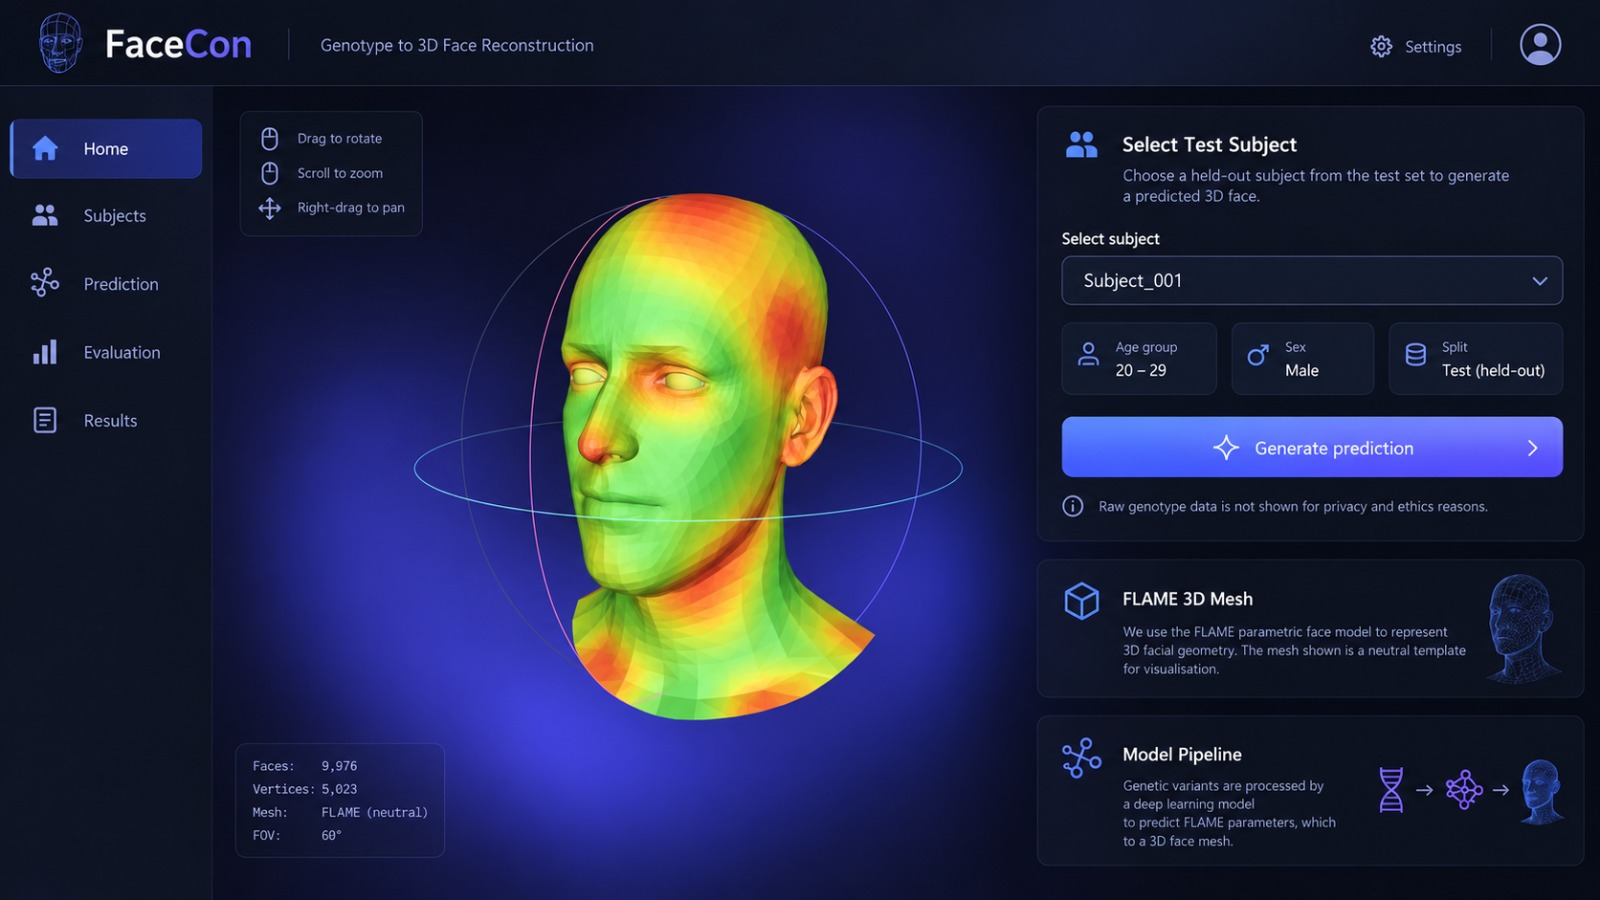
\includegraphics[width=\textwidth]{Figures/ui_selection.png}
\caption{Test subject selection screen (UC-04).}
\label{fig:ui1}
\end{figure}

\begin{figure}[!ht]
\centering
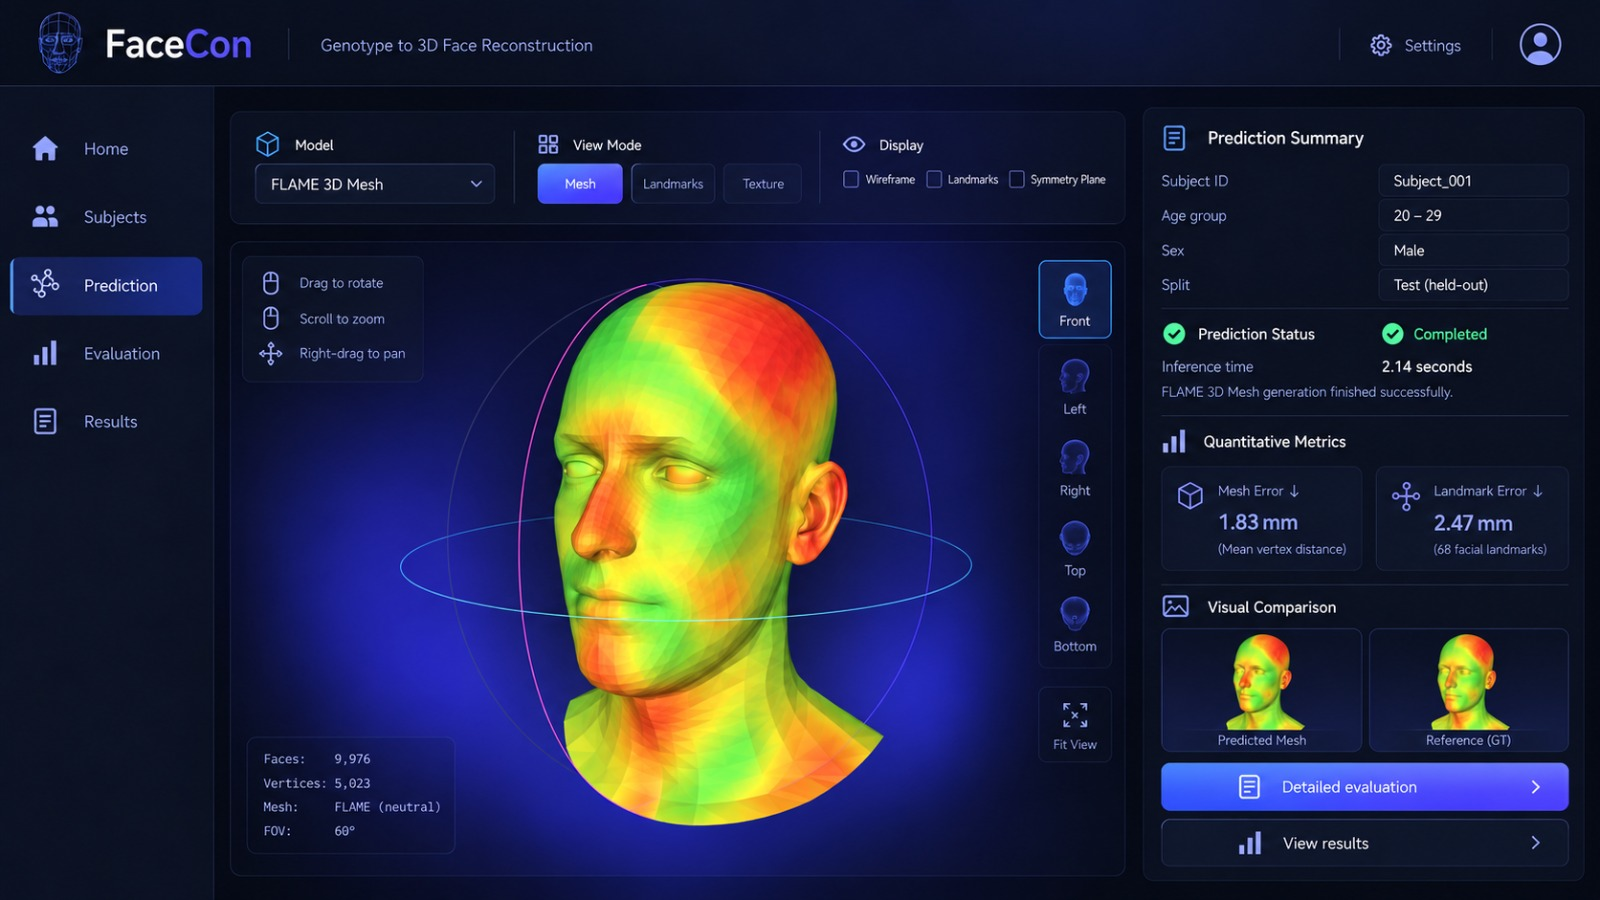
\includegraphics[width=\textwidth]{Figures/ui_comparison.png}
\caption{Prediction screen (UC-05).}
\label{fig:ui2}
\end{figure}

\begin{figure}[!ht]
\centering
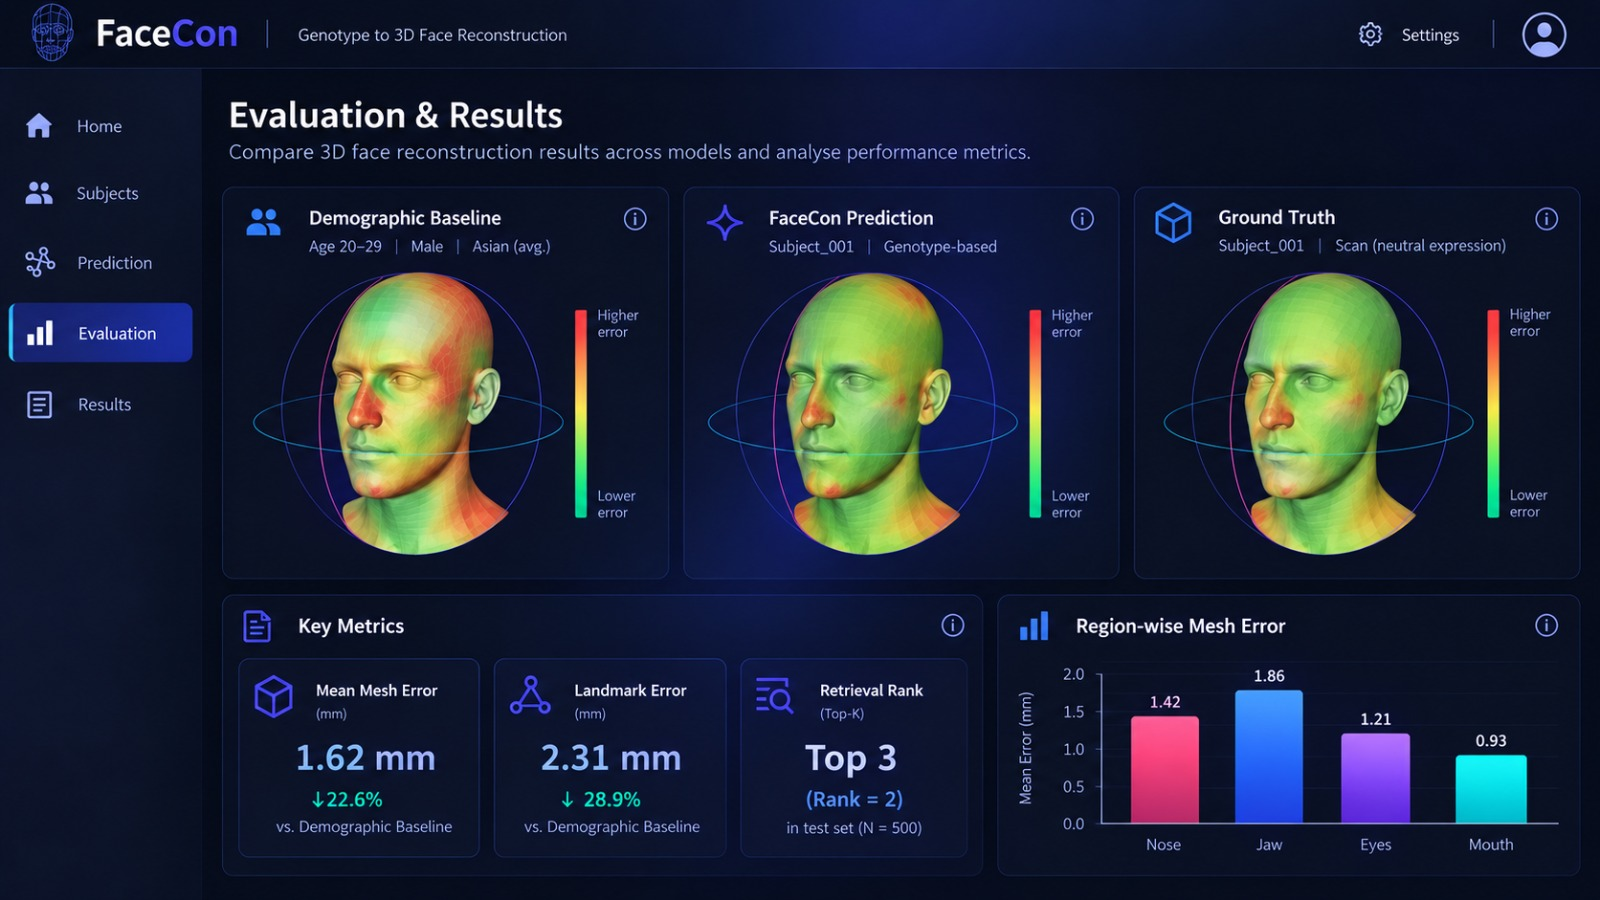
\includegraphics[width=\textwidth]{Figures/ui_detailed.png}
\caption{Evaluation and results screen (UC-06).}
\label{fig:ui3}
\end{figure}

\begin{figure}[!ht]
\centering
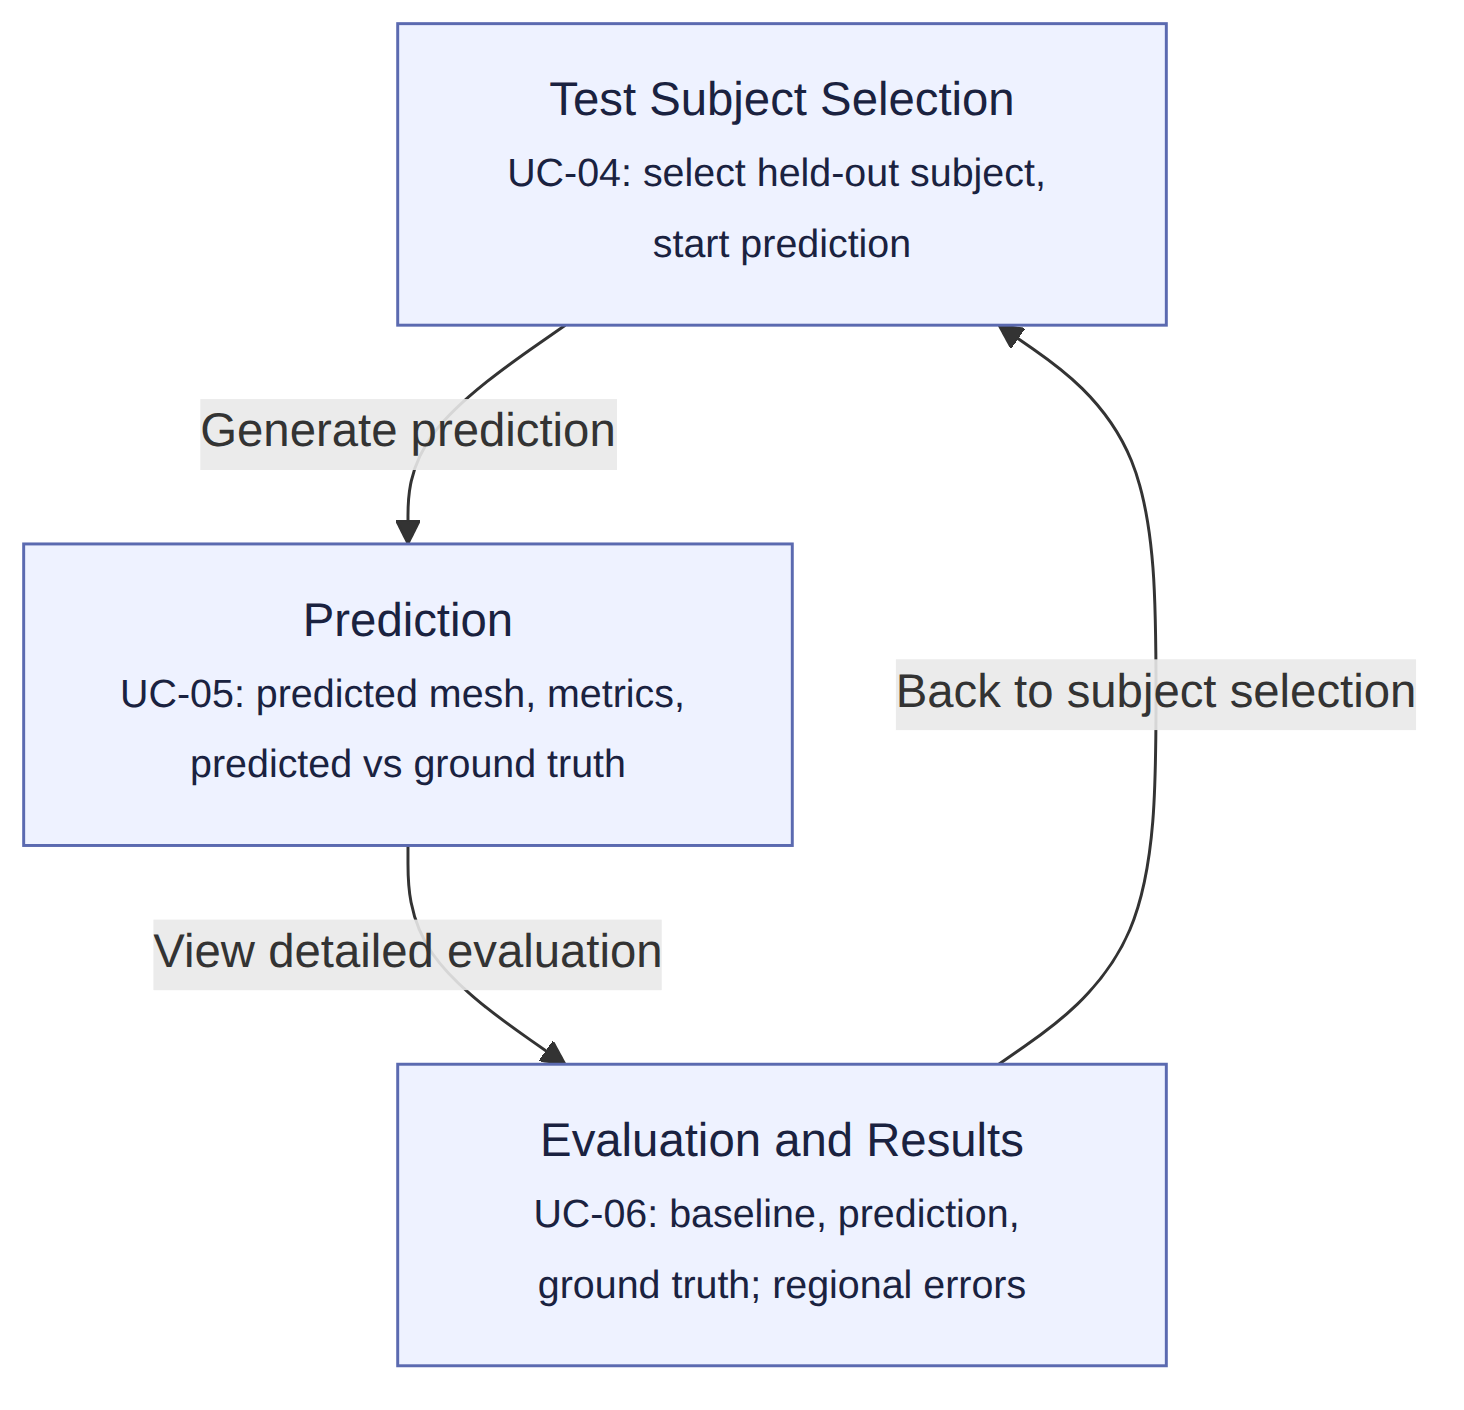
\includegraphics[width=0.5\textwidth]{Figures/nav.png}
\caption{Navigation flow of the demonstrator.}
\label{fig:nav}
\end{figure}

The mapping between the demonstrator screens and the use cases and functional requirements is as follows. Screen 1, test subject selection, realizes UC-04 and starts prediction through FR-06. Screen 2, prediction, realizes UC-05 and exercises FLAME decoding (FR-07) and evaluation (FR-08), presenting the predicted mesh, its metrics, and a comparison with the ground truth. Screen 3, evaluation and results, realizes UC-06 and exercises evaluation and baseline comparison (FR-08, FR-09), presenting the demographic baseline, the prediction, and the ground truth together with regional errors. Because the demonstrator displays a ground truth FLAME face alongside the prediction, it relies on the held-out FLAME targets produced by the registration stage (FR-04), which are available for evaluation but never used during training.

\section{Database Design}
FaceCon is data-centric rather than transaction-centric, so it stores structured, file artifacts rather than using a relational database. No SQL or entity-relationship schema is therefore required. The data design and dictionary are nonetheless documented.

\subsection{Data Dictionary}
Table~\ref{tab:datadict} is the data dictionary for the principal FaceCon artifacts, keyed by de-identified subject identifiers.

\begin{table}[!ht]
\centering
\caption{Data dictionary for the principal FaceCon data artifacts.}
\label{tab:datadict}
\small
\begin{tabular}{|P{2.6cm}|P{2.6cm}|P{2.2cm}|P{5.4cm}|}
\hline
\textbf{Entity} & \textbf{Field} & \textbf{Type} & \textbf{Description} \\ \hline
Subject & subject\_id & String & De-identified key linking genotype and scan. \\ \hline
Genotype & snp\_dosage & Int matrix & Allele dosages (0/1/2) for the documented SNP panel. \\ \hline
Genotype & qc\_flags & Struct & Per-subject QC outcomes and imputation notes. \\ \hline
FaceShape & flame\_params & Float array & FLAME identity/shape parameters from fitting. \\ \hline
FaceShape & fit\_error & Float & Registration error between scan and FLAME mesh. \\ \hline
Appearance & colour\_outputs & Categorical & Eye colour, hair colour, and skin colour returned by the integrated HIrisPlex-S predictor. \\ \hline
Appearance & hirisplex\_markers & Int matrix & Allele dosages for the HIrisPlex-S marker SNPs extracted from the genotype. \\ \hline
Demographics & age, gender, ancestry/PCs & Mixed & Covariates for baselines and stratification. \\ \hline
Split & split\_label & Enum & Train / validation / test assignment. \\ \hline
Prediction & pred\_params & Float array & Predicted FLAME shape for a subject. \\ \hline
Prediction & baseline\_params & Float array & Demographic-baseline FLAME shape for comparison. \\ \hline
\end{tabular}
\end{table}

\section{Risk Analysis}
This section identifies the main risks to the project, together with their category, cause, potential impact, likelihood, severity, and the mitigation and contingency measures planned for each. Because FaceCon is a research and development project that depends on controlled-access data and uncertain experimental outcomes, the most significant risks are concentrated in the data, methodological, and evaluation categories rather than in conventional software-failure categories. Table~\ref{tab:risk} summarizes the analysis.

{\footnotesize\setlength{\LTpre}{6pt}\setlength{\LTpost}{0pt}
\begin{longtable}{|P{2.5cm}|P{3.3cm}|P{2.5cm}|P{1.6cm}|P{3.0cm}|}
\caption{Risk analysis for the FaceCon project.}\label{tab:risk}\\
\hline
\textbf{Risk / Category} & \textbf{Description and Cause} & \textbf{Potential Impact} & \textbf{Likelihood / Severity} & \textbf{Mitigation and Contingency} \\ \hline
\endfirsthead
\hline
\textbf{Risk / Category} & \textbf{Description and Cause} & \textbf{Potential Impact} & \textbf{Likelihood / Severity} & \textbf{Mitigation and Contingency} \\ \hline
\endhead
\hline
\endfoot
Delayed or denied data access \newline (Access / Data) & Approval for dbGaP and FaceBase may be slow or refused, owing to institutional review and data-use-agreement processes. & Training on real data is blocked and the schedule may slip. & Medium / High & Develop and validate the pipeline on synthetic data in parallel. Contingency: continue methodological and synthetic-data work and escalate the access request. \\ \hline
Small usable paired-sample size \newline (Data / Methodological) & Few subjects may have both a genotype and a valid 3D scan after QC, because of scarcity and filtering. & Low statistical power and a tendency for complex models to overfit. & High / High & Prefer simple, regularized models and strong baselines, and report confidence intervals. Contingency: restrict scope to baselines and report limits honestly. \\ \hline
Poor scan to FLAME fitting \newline (Data quality / Preprocessing) & Some scans may register poorly to FLAME, owing to noise, missing regions, or landmark errors. & Label noise in training targets and biased evaluation. & Medium / Medium & Enforce fitting-error thresholds and exclude or flag poor fits. Contingency: correct landmarks manually or exclude the subject with documentation. \\ \hline
Demographic and population confounding \newline (Methodological / Evaluation) & Age, gender, and ancestry drive facial variation and can inflate apparent genotype accuracy. & Overstated individual-level genetic contribution. & High / Medium & Evaluate demographic-only, genotype-only, and combined models and report the incremental gain. Contingency: stratified analysis and explicit reporting of confounding. \\ \hline
Data leakage across splits \newline (Methodological / Evaluation) & Subjects or fitted statistics could leak between splits through relatedness or statistics fitted on all data. & Optimistic, irreproducible results. & Medium / High & Use subject-level splits that respect relatedness and fit statistics on training folds only. Contingency: re-run with corrected splits and discard affected results. \\ \hline
Overfitting of complex models \newline (Modelling) & High-dimensional SNP inputs relative to a small sample encourage memorization. & Misleadingly low training error and poor generalization. & Medium / Medium & Follow the baselines first progression with regularization and early stopping, matching complexity to the data. Contingency: fall back to simpler models. \\ \hline
Ancestry bias and limited generalization \newline (Research / Data) & GWAS priors and the cohort are skewed toward specific ancestries. & Results may not transfer to other populations. & Medium / Medium & Document provenance and stratify by ancestry where possible. Contingency: scope conclusions to the evaluated population. \\ \hline
Integration and reproducibility drift \newline (Integration / Reproducibility) & Dependency, seed, or configuration changes across environments. & Non-reproducible results and wasted effort. & Low / Medium & Pin dependencies, fix seeds, and capture per-run configurations. Contingency: restore the exact recorded configuration. \\ \hline
Schedule compression \newline (Schedule) & Research uncertainty and data delays reduce the available time. & Incomplete experiments by the deadline. & Medium / Medium & Prioritize baselines and core evaluation and treat advanced models as stretch goals. Contingency: descope the advanced generative stage. \\ \hline
\end{longtable}
}

\section{Conclusion}
This chapter has specified what FaceCon must do and how well it must do it. The features were turned into functional requirements written in a testable form, so that each can be traced to a test case in Chapter~\ref{ch:impl}, and the non-functional requirements fixed the properties that matter most for a research system of this kind: reproducibility, protection of controlled-access data, and the separation of training data from everything used to judge a model. The use cases describe how a user selects a held-out subject, generates a prediction, and compares it with the demographic baseline and the ground truth, and the interface designs give those use cases a concrete form. The data design records the artefacts the pipeline produces in a data dictionary rather than a relational schema, since FaceCon stores structured files and not transactions. The risk analysis anticipated the most serious problem the project met, the delay in data access, and its mitigation, a simulated cohort, is what made the rest of this phase possible. The next chapter develops the methodology that meets these requirements.
